\documentclass[pdflatex,sn-basic]{sn-jnl}

\usepackage{amsmath,amssymb}
\usepackage{bm}
\usepackage{graphicx}
\usepackage{booktabs}
\usepackage{array}
\usepackage{textcomp}
\usepackage{xcolor}
\usepackage{manyfoot}
\usepackage[section]{placeins}

\raggedbottom

\begin{document}

\title[Conservative DBS Formulation for PHREEQC-Coupled Reactive Transport]{A Conservative Darcy-Brinkman-Stokes Formulation for PHREEQC-Coupled Reactive Transport with Cell-Based Surface Complexation}

\author*[1,2]{\fnm{Hannah P.} \sur{Menke}}\email{H.Menke@hw.ac.uk}

\author[1,2]{\fnm{Florian} \sur{Doster}}

\author[1,2]{\fnm{Julien} \sur{Maes}}

\affil*[1]{\orgdiv{Institute for GeoEnergy Engineering}, \orgname{Heriot-Watt University}, \orgaddress{\city{Edinburgh}, \country{United Kingdom}}}

\affil[2]{\orgdiv{SET-IT (Subsurface Energy Transition \& Innovation Centre)}, \orgname{Heriot-Watt University}, \orgaddress{\city{Edinburgh}, \country{United Kingdom}}}

\begin{abstract}
This draft presents a diffuse-boundary-surface (DBS) formulation for
PHREEQC-coupled reactive transport with cell-based surface complexation. The
model is designed to preserve conservative aqueous transport in the mobile
water fraction, retain a local conservative exchange between dissolved and
adsorbed inventories, and avoid non-conservative numerical fixes such as
species clipping. The implementation is built in stages from validated
reductions, culminating in a production solver for DBS transport with optional
surface complexation.

The paper is organized around a validation ladder: a 1D analytical benchmark,
a simple 2D image-based case, a simple 3D image-based case, and a larger 3D
porous-media demonstration. The current draft already includes a passing 1D
analytical retardation benchmark, a corrected 2D fracture-network result with
matrix-wide unresolved surface uptake, and a reserved 3D Kelvin figure slot
with a tracked runtime case behind it. The large multi-scale Estaillades-style
case now also has a corrected
production run with reported timing and field metrics; only its final 3D
volume-rendered figure is still blocked by the current ParaView headless
rendering environment. The manuscript intentionally omits final references so the
mathematical statement, implementation details, and test-case results can be
stabilized first.
\end{abstract}


\keywords{Darcy-Brinkman-Stokes, PHREEQC, surface complexation, micro-continuum reactive transport, image-based porous media, direct lithium extraction}

\maketitle

\noindent\textbf{Article Highlights}
\begin{itemize}
\item A cell-based method links pore-scale flow, solute transport, and surface chemistry.
\item Dissolved and surface-bound species enter the same local mass balance.
\item One surface-area field combines visible interfaces with unresolved internal area.
\end{itemize}

\section{Introduction}

Surface complexation is a key control on reactive transport in porous media,
but most pore-scale implementations assume either explicitly resolved grain
surfaces or simplified source terms that are not tied cleanly to a
conservative transport balance. The objective of this work is to develop a DBS
formulation that couples PHREEQC chemistry to unresolved internal surface area
while preserving mathematically correct inventory balances.

The guiding constraints of this implementation are:
\begin{itemize}
\item the transport equation must conserve mobile aqueous inventory in the
physical mobile-water fraction,
\item local chemistry must conserve total inventory while transferring mass
between aqueous and adsorbed states,
\item the baseline method must not rely on concentration clipping, damping, or
heuristic face-based reaction reconstruction.
\end{itemize}

The solver developed in this work is \texttt{reactiveScalarTransportDBSFoam}.
It is built on a staged validation program so every major reduction path
remains testable. This manuscript follows the same overall structure as the
earlier GeoChemFoam reactive transport paper: introduction, model description,
implementation, validation, and then progressively more complex test cases.

\section{Model Description}
\label{sec:model}

\subsection{Field Definitions}

The DBS micro-continuum formulation \citep{brinkman1949calculation,soulaine2016micro,
soulaine2024microcontinuum} represents the pore medium as a continuum in which
a cell-centred porosity field $\epsilon$ varies smoothly from
zero (solid) to unity (open pore). The steady incompressible flow is governed
by the Darcy-Brinkman equations:
\begin{align}
\nabla \cdot \bm{u}_D &= 0,
\label{eq:continuity} \\
-\nabla p + \nabla \cdot \bigl(\mu_{\mathrm{eff}} \nabla \bm{u}\bigr)
- \frac{\mu}{K(\epsilon)}\,\bm{u}_D &= \bm{0},
\label{eq:brinkman}
\end{align}
where $\bm{u}_D = \epsilon\bm{u}$ is the Darcy velocity,
$\mu$ is the fluid viscosity, $\mu_{\mathrm{eff}}$ is an effective
viscosity that smoothly recovers the Stokes equation in open-pore cells
\citep{soulaine2016micro}, and $K(\epsilon)$ is a permeability
function. The drag coefficient $\mu/K(\epsilon)$ therefore acts
as a large resistance term in solid-like cells and vanishes in open-pore cells,
so Eq.~\eqref{eq:brinkman} reduces to the Stokes equation.

For an image-derived cell, let $f_k$ be the geometric fraction of source voxels
assigned to segmented phase $k$, with $\sum_k f_k=1$, and let $\phi_k$ be the
end-member porosity assigned to that phase. The cell DBS porosity is
\begin{equation}
\epsilon=\sum_k f_k\phi_k.
\label{eq:phase_porosity}
\end{equation}
The fraction $f_k$ describes phase occupancy, whereas $\phi_k$ specifies the
water-filled fraction of that phase. A cell wholly occupied by a microporous
phase therefore has $f_{\mathrm{micro}}=1$ and
$\epsilon=\phi_{\mathrm{micro}}<1$. Nominal solid is assigned a small non-zero
porosity as a numerical DBS floor.

The mobile-water fraction $\theta$ is the mobile-water volume per bulk cell
volume. It governs aqueous storage, diffusion, and PHREEQC solution volume,
whereas $\epsilon$ governs DBS flow resistance and relates intrinsic velocity
to Darcy velocity. The saturated calculations reported here set
$\theta=\epsilon$ in chemically active cells. Cells with
$\theta\leq\theta_{\mathrm{mask}}$ are excluded from chemistry.

Reactive surface area is specified independently as the cell-centred bulk-volume
density $a_{\mathrm{surf}}$ (m$^2$\,m$^{-3}_{\mathrm{bulk}}$). All aqueous
species, $\theta$, $a_{\mathrm{surf}}$, and adsorbed surface fields are
cell-centred; transport fluxes are evaluated on cell faces.

\subsection{Reactive Surface Area Field}
\label{sec:aSurf}

Reactive area is present only for selected interfaces and phases assigned a
non-zero intrinsic density. Its resolved and unresolved contributions are
carried in the fixed cell-centred field $a_{\mathrm{surf}}$ (units:
m$^2\,\mathrm{m}^{-3}_{\mathrm{bulk}}$), the sum of two terms:
\begin{equation}
a_{\mathrm{surf}} = a_{\mathrm{surf}}^{\mathrm{interface}} +
a_{\mathrm{surf}}^{\mathrm{intrinsic}}.
\label{eq:asurf}
\end{equation}

The interface term is reconstructed for an ordered pair of segmented labels.
One label is the owner and the second is the other phase; their union restricts
the extracted interface, and the owner identifies the side used for area
assignment. In \texttt{occupancyGaussian}, the Gaussian-filtered owner
indicator is normalised by the Gaussian-filtered pair mask, and the $0.5$
level is extracted.

Three-dimensional triangle area is divided by bulk cell volume to obtain
$a_{\mathrm{surf}}^{\mathrm{interface}}$. In quasi-two-dimensional images,
contour length is multiplied by physical out-of-plane thickness before
division by cell volume. For quasi-two-dimensional cell-field construction,
\texttt{occupancyGaussian} uses weighted redistribution over owner-side
first-shell contact cells. Pieces with empty support contribute zero area
to the deposited field. Detailed support and partition rules are given in
Online Resource~1.

\begin{table*}[htbp]
    \centering
    \caption{Interface reconstruction parameters. All cases use
    \texttt{occupancyGaussian} with an isovalue of $0.5$.
    The ordered pair is owner $\rightarrow$ other; the owner defines the
    indicator used for reconstruction. In cell-field constructions,
    reconstructed area is assigned on the owner side.}
    \label{tab:surfaceConstruction}
    \scriptsize
    \setlength{\tabcolsep}{3pt}
    \begin{tabular}{@{}p{0.28\textwidth}p{0.12\textwidth}p{0.48\textwidth}@{}}
        \toprule
        Case & $\sigma$ (vox) & Pair (owner $\rightarrow$ other) \\
        \midrule
        Circular post & 1.50
            & exterior/pore 255 $\rightarrow$ post/solid 0 \\
        Sphere & 0.75
            & exterior/pore 255 $\rightarrow$ sphere/solid 0 \\
        HM12 solid-grain DBS & 0.75
            & pore 255 $\rightarrow$ solid 0 \\
        2D four-fracture & 0.75
            & micropore 1 $\rightarrow$ pore 2 \\
        3D Kelvin & 0.75
            & micropore 2 $\rightarrow$ pore 1 \\
        3D Estaillades & 0.74
            & pore 1 $\rightarrow$ solid 3 \\
        3D external area & 0.74
            & pore 1 $\rightarrow$ remapped solid 3 \\
        \bottomrule
    \end{tabular}
\end{table*}

The interface term captures only boundaries between grain and fluid that are
visible at the resolved image scale. It does not detect
reactive area that lies entirely \emph{within} a voxel, such as sub-voxel
surface roughness of a grain or the internal pore network of a microporous
phase. Those surfaces are below the image resolution by construction.

The second term, $a_{\mathrm{surf}}^{\mathrm{intrinsic}}$, accounts for this
sub-voxel contribution. An end-member surface density $s_k$
(units: m$^2$\,m$^{-3}_{k}$) is prescribed per unit volume of each segmented
phase $k$ (for example pore, micropore, or dense solid). It may represent
sub-voxel surface such as the
Brunauer-Emmett-Teller (BET) surface area of a microporous grain measured by
N$_2$ adsorption, or the surface roughness of a dense solid grain measured on
powdered material. Mass-specific measurements are converted to phase-volume
densities using the corresponding mass per unit phase volume.

The intrinsic contribution is assembled by weighting each phase density by
its geometric fraction $f_k$ within the computational cell:
\begin{equation}
a_{\mathrm{surf}}^{\mathrm{intrinsic}} = \sum_k f_k\,s_k.
\label{eq:asurf_intrinsic}
\end{equation}
Thus $f_k$ converts the phase-volume density $s_k$ to a bulk-volume cell
contribution. A density already expressed per bulk cell volume represents
that contribution directly. The segmented image supplies $f_k$, whereas
$s_k$ is prescribed from complementary measurements or finer-scale
characterisation.

$s_k$ may be non-zero for any label, including labels selected for interface
reconstruction. The same segmented label may contribute through both terms:
$a_{\mathrm{surf}}^{\mathrm{interface}}$ gives the image-scale outer surface
of the grain, and $a_{\mathrm{surf}}^{\mathrm{intrinsic}}$ adds the
sub-voxel surface area that the image resolution cannot capture. If
$s_k=0$ for all labels, the total reduces to the purely geometric image-scale
surface. Both contributions are pre-computed using the segmented image and
prescribed phase properties before the flow simulation begins and are held
constant throughout the reactive-transport calculation.

Both contributions enter the geochemical module through the same bulk-volume
field. The \texttt{phreeqcMixture} builds used for the reported calculations
supply surface area per representative bulk litre to PHREEQC as
\begin{equation}
a_{\mathrm{surf}}^{\mathrm{bulk,L}} = \frac{a_{\mathrm{surf}}}{10^{3}},
\label{eq:asurf_bulk_litre}
\end{equation}
For surface master $k$, the site density $N_k$ (mol\,m$^{-2}$) gives a
surface-master inventory per bulk volume of $N_k a_{\mathrm{surf}}$
(mol\,m$^{-3}_{\mathrm{bulk}}$). These conversions use the bulk-volume basis
without division by $\theta$.

Surface areas estimated from nano-computed tomography
(nano-CT), micro-computed tomography (micro-CT), focused ion beam scanning
electron microscopy (FIB-SEM), or other image data are first expressed on a
bulk-volume basis (m$^2$\,m$^{-3}_{\mathrm{bulk}}$), consistent with
Eqs.~\eqref{eq:asurf} and~\eqref{eq:asurf_intrinsic}. Image-derived surface areas
reported per microporous-phase volume or per grain mass are converted to this
bulk-volume basis before Eq.~\eqref{eq:asurf_bulk_litre} is applied.

The same fixed porosity field is used for DBS transport and for the PHREEQC
solution volume. Cells in
which $\theta$ falls below the chemistry mask threshold
$\theta_{\mathrm{mask}}$ are treated as chemically inactive and their surface
terms are suppressed.

\subsection{Conservative Aqueous Transport}

For each aqueous species with concentration $C_i$, the conservative DBS
transport equation is written as
\begin{equation}
\frac{\partial (\theta C_i)}{\partial t}
+ \nabla \cdot (\bm{u}_D C_i)
- \nabla \cdot (\theta D_i \nabla C_i) = 0,
\end{equation}
where $\bm{u}_D$ is the Darcy velocity satisfying
Eqs.~\eqref{eq:continuity} and~\eqref{eq:brinkman}, and $D_i$ denotes the
diffusivity used in the transport equation. In fully resolved macro-pore cells
($\theta \approx 1$), $D_i$ is the free molecular diffusivity. In cells that
represent microporous material ($0 < \theta < 1$), $D_i$ is interpreted as an
effective diffusivity, commonly $D_i = D_i^{\mathrm{mol}}/\tau$, where
$D_i^{\mathrm{mol}}$ is the molecular diffusivity and $\tau \geq 1$ is the
tortuosity factor of the micropore network. In either case, the $\theta$ factor
multiplying $D_i$ in the diffusion term accounts for the reduced water volume
available for transport. Reactions enter through the operator-split PHREEQC
step described below, not as a source term in this equation.

For a vector of aqueous species $\bm{C}$, the same balance is
\begin{equation}
\frac{\partial (\theta \bm{C})}{\partial t}
+ \nabla \cdot (\bm{u}_D \bm{C})
- \nabla \cdot (\theta \bm{D} \nabla \bm{C}) = \bm{0},
\end{equation}
where $\bm{D}$ collects the species diffusivities. This notation is used for
the split operators below.

\subsection{Cell-Based Surface Inventory}

For the cell-based unresolved surface carried by the DBS formulation, the
conservative local inventory is expressed
in the current solver field variables as
\begin{equation}
M = \theta C + a_{\mathrm{surf}}\Gamma,
\label{eq:inventory}
\end{equation}
where $\Gamma$ is the cell-centred surface-species concentration
(mol\,m$^{-2}$ of reactive surface). The first term is the aqueous amount per
bulk volume, the second the adsorbed amount per bulk volume. Porosity enters
the aqueous term once, and the bulk-based surface-area field carries no
porosity scaling.

For multiple surface species the local bulk inventory is the sum of the aqueous
and adsorbed contributions over species; single-species notation is used
below.

\subsection{Local Chemistry Coupling}

The chemical update is local to each cell. Over one cycle of transport and
chemistry, the transport step first advances the aqueous species in
conservative finite-volume form. The updated cell state, together with the mobile-water
fraction and cell-based surface state, is then mapped into PHREEQC
\citep{parkhurst2013phreeqc} via the PhreeqcRM interface
\citep{parkhurst2015phreeqcrm}. PHREEQC solves the local chemistry at
\emph{thermodynamic equilibrium}, treating surface complexation as
instantaneous relative to transport within each timestep. This holds when the
surface equilibration time is short compared with the time for advection and
diffusion across a cell. The same interface supports kinetic surface reactions,
which are not used here.

The solver uses first-order Lie splitting \citep{carrayrou2004operator}. The
splitting introduces a global error of $\mathcal{O}(\Delta t)$ in the
operator-split solution; the local error over one step is
$\mathcal{O}(\Delta t^2)$. For the timesteps used here, the advective
Courant-Friedrichs-Lewy (CFL) number remains $O(1)$, so the
operator-splitting error is of the same formal order as the first-order
transport discretisation. The resulting algorithm keeps the conservative
transport update and the local PHREEQC equilibrium update as distinct
operators within each timestep.

At the algorithmic level, one timestep of size $\Delta t$ is:
\begin{align}
\widetilde{\bm{C}}^{\,n+1} &= \mathcal{T}_{\Delta t}(\bm{C}^{n}, \theta, \bm{u}_D, \bm{D}),\\
(\bm{C}^{n+1}, \bm{\Gamma}^{n+1}) &=
\mathcal{R}_{\Delta t}(\widetilde{\bm{C}}^{\,n+1}, \bm{\Gamma}^{n}, \theta, a_{\mathrm{surf}}),
\end{align}
where $\mathcal{T}_{\Delta t}$ is the conservative finite-volume transport
operator (advancing $\theta\bm{C}$ in DBS form) and $\mathcal{R}_{\Delta t}$
is the local PHREEQC equilibrium operator that updates both aqueous and
surface states simultaneously within each cell.

\subsection{Analytical Dilute Limit}

In the dilute linear-equilibrium limit, surface complexation reduces to a
Henry-type isotherm. The standard Henry coefficient is $K_s = \Gamma / C$
(units: m), the ratio of surface concentration $\Gamma$ (mol\,m$^{-2}$) to
aqueous concentration $C$ (mol\,m$^{-3}$):
\begin{equation}
\Gamma = K_s C.
\end{equation}
$K_s$ is obtained from a pair of batch equilibrations at two aqueous
concentrations, $K_s = \Delta\Gamma / \Delta C$, which returns the coefficient
in the field units used by the retardation formula.

Substituting into the inventory Eq.~\eqref{eq:inventory} and taking the
time derivative yields the retarded 1D transport equation
\begin{equation}
\left(
\theta + a_{\mathrm{surf}}K_s
\right)\frac{\partial C}{\partial t}
+ \frac{\partial (u_D C)}{\partial x} = 0.
\end{equation}
The corresponding retardation factor is
\begin{equation}
R = 1 + \frac{a_{\mathrm{surf}}\,K_s}{\theta}.
\label{eq:retardation}
\end{equation}
Both $a_{\mathrm{surf}}$ and $\theta$ can vary spatially, so
Eq.~\eqref{eq:retardation} also gives the local retardation at any point in
a heterogeneous domain. The classical semi-infinite advection--diffusion
solution follows \citet{ogata1961solution}. For comparison with the finite 1D
calculation, the reference problem is instead evaluated on $[0,L]$ with the
same fixed-concentration inlet and zero-gradient outlet as the numerical case,
using the effective velocity $u_D/(\theta R)$ and diffusivity $D/R$.

\section{Numerical Implementation}

The numerical implementation couples conservative DBS transport with
cell-centred PHREEQC chemistry and cell-based surface complexation in a single
operator-split formulation. The discussion below describes the discrete fields,
the transport--chemistry coupling, and the timestep algorithm used in the
reported simulations.

\subsection{Field Locations And Discretization}

The baseline discretization keeps all chemistry-bearing state cell-centered.
This avoids introducing an extra face reconstruction for the unresolved
surface-reaction source. The solution species, $\theta$,
$\epsilon_{\mathrm{num}}$, $a_{\mathrm{surf}}$, and the surface fields are
therefore stored at cell centres, whereas only the volumetric flux $\phi$
remains face-centred. Transport uses face interpolation only within the
conservative flux assembly, while the surface chemistry remains strictly
cell-local.

For microporous image cases, the current implementation treats the cell-centered
surface-area field as an additive quantity:
\[
    a_{\mathrm{surf}} =
    a_{\mathrm{surf}}^{\mathrm{interface}} +
    a_{\mathrm{surf}}^{\mathrm{intrinsic}}.
\]
The first term is the coarse-grained phase-boundary contribution. The second is
an intrinsic volumetric surface density assigned to selected image phases
(for example the micropore phase) and scaled by the corresponding local phase
fraction inside each coarse cell.

\subsection{PHREEQC Coupling}

The PHREEQC coupling is performed through \texttt{phreeqcDBSMixture}. For each
cell, the coupling uses the current aqueous state, the physical mobile-water
fraction $\theta$, the current cell surface area $a_{\mathrm{surf}}$ including
any intrinsic micropore contribution, and the current cell surface state. The
surface mode is optional and reduces exactly to aqueous-only mode when
$a_{\mathrm{surf}} = 0$.

Cells with negligible mobile-water fraction remain chemically inactive in the
written finite-volume state. In the current implementation this is enforced at
the field level, even though the PHREEQC backend may still use an internal
dummy water volume to keep the chemistry module numerically well-posed.

\subsection{Per-Timestep Algorithm}

The production timestep is intentionally simple. At each step, the solver reads
or updates the face flux $\phi$, advances each aqueous transport equation in
conservative DBS form, pushes the updated cell state into PHREEQC, executes
the local chemistry update, pulls the updated aqueous and surface states back
into the finite-volume fields, and finally writes diagnostics, including
integrated inventory summaries. This is the appropriate baseline for a first
conservative implementation because the transport and chemistry operators
remain individually testable.

\begin{figure}[htbp]
    \centering
    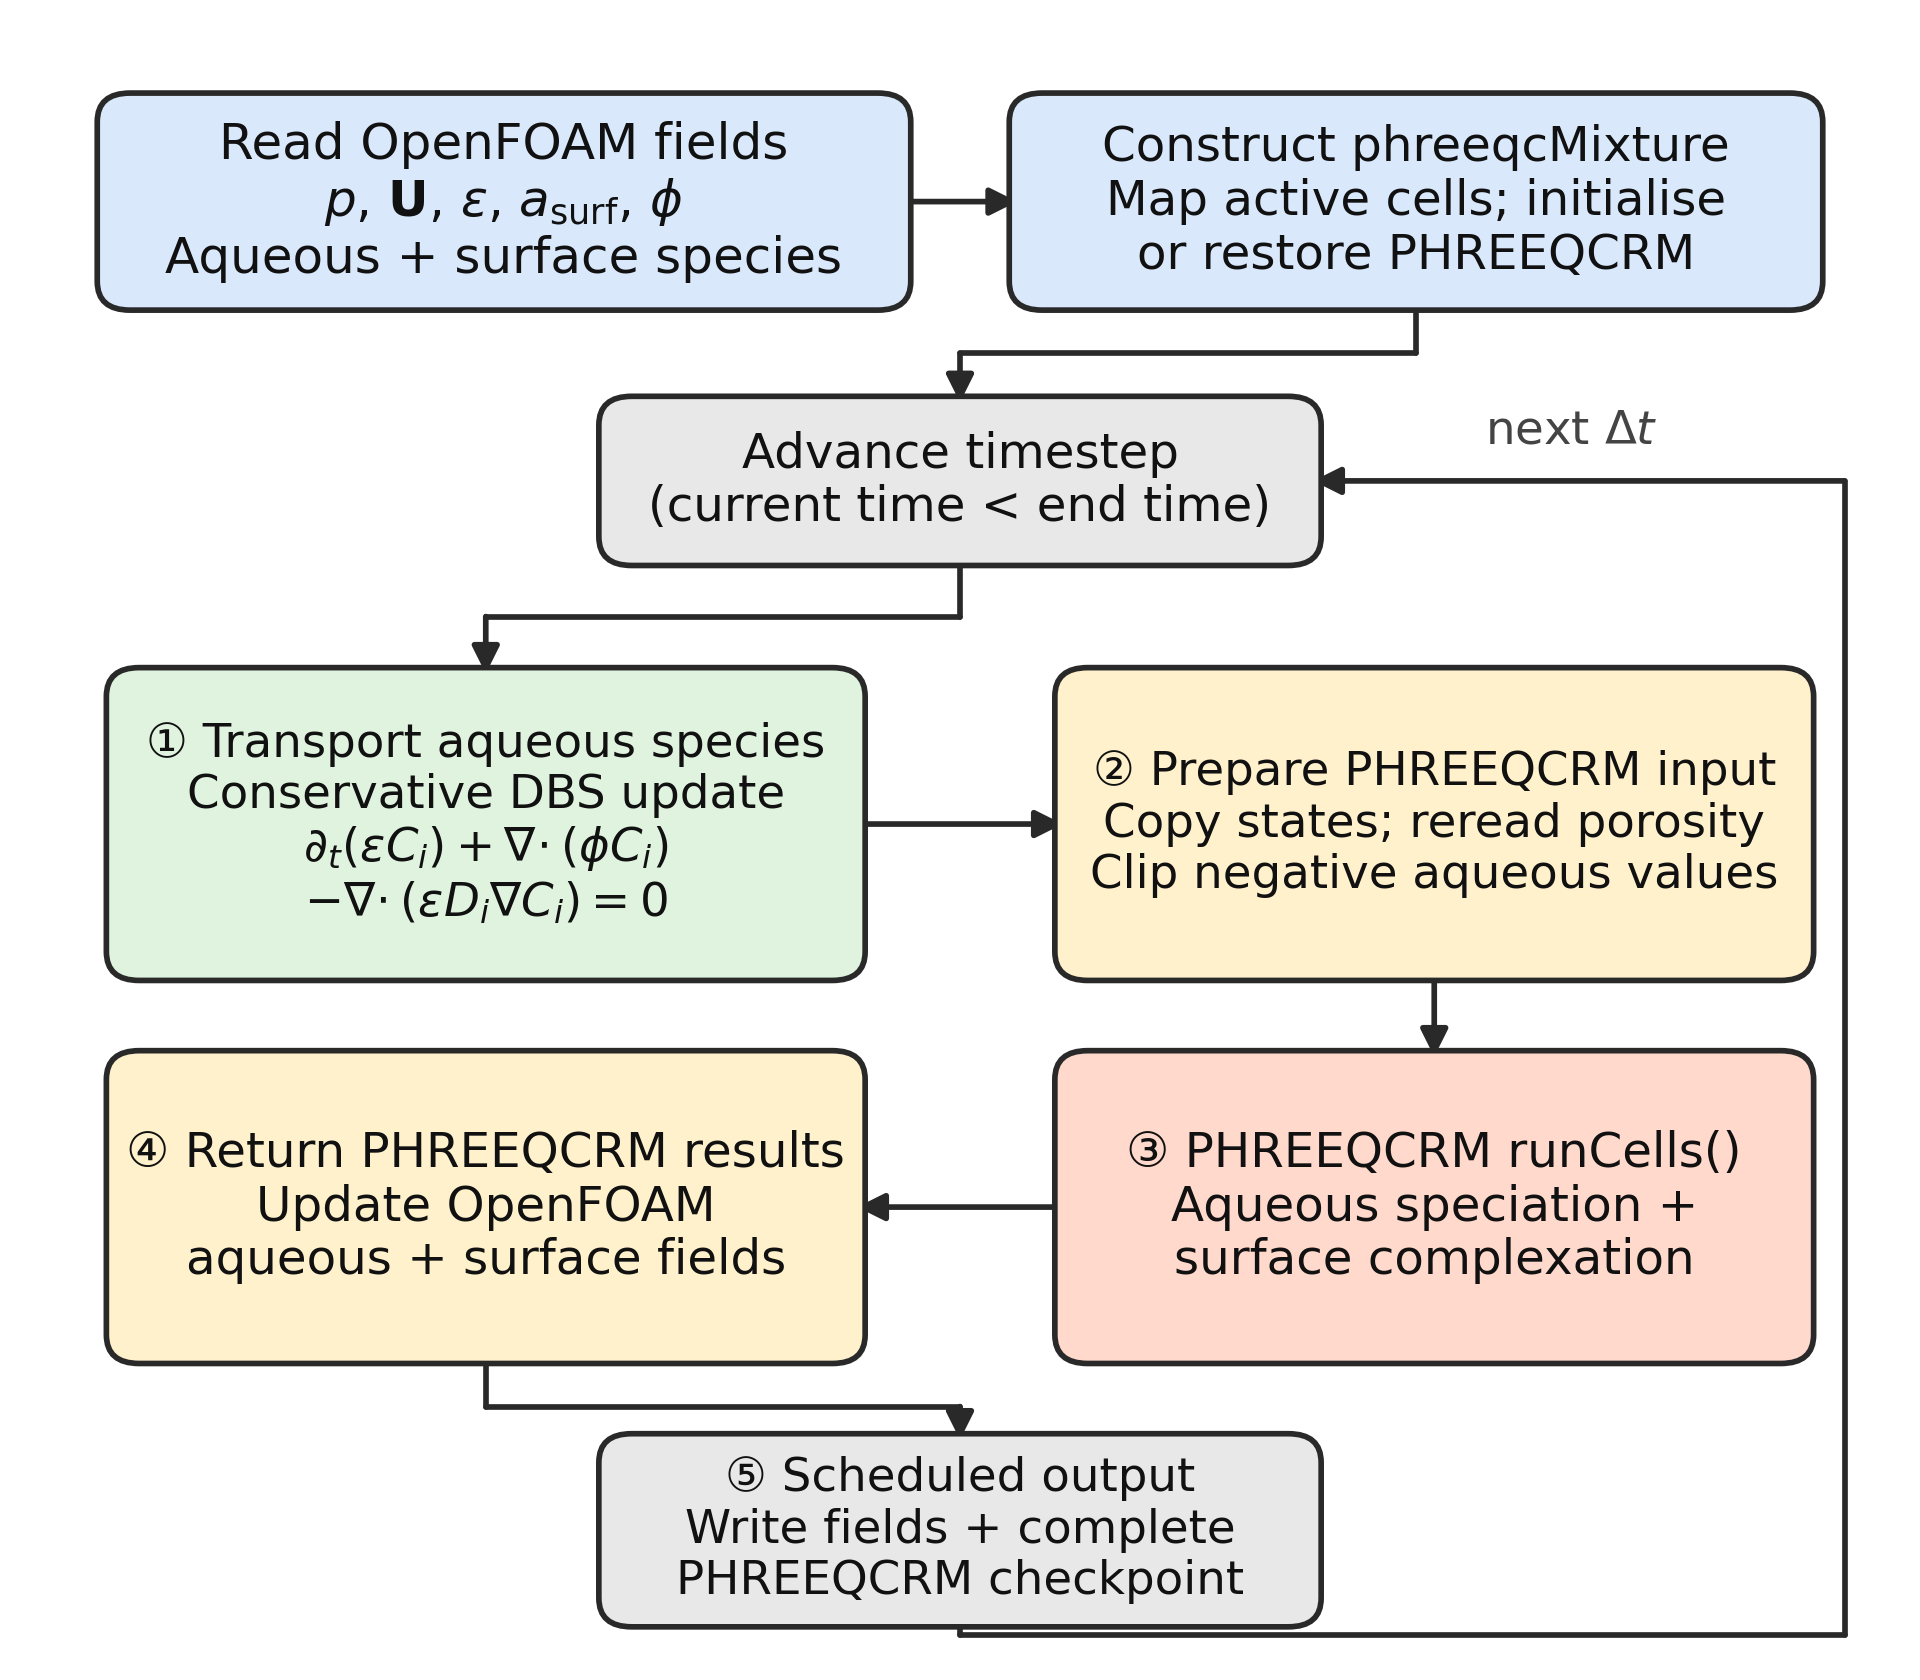
\includegraphics[width=0.96\linewidth]{figures/png/fig05_solver_workflow.png}
    \caption{Full solution procedure for
    \texttt{reactiveScalarTransportDBSFoam}. The solver reads the current
    finite-volume state, initializes or updates the cell-based PHREEQC
    coupling through \texttt{phreeqcDBSMixture}, advances all aqueous species
    in conservative DBS form, executes the local cellwise chemistry update,
    and then writes the updated aqueous and surface states back to the
    finite-volume fields. The workflow is intentionally operator-split:
    transport is solved first, followed by local PHREEQC chemistry, so the two
    operators remain independently testable and the conservative structure of
    the aqueous transport step is never hidden inside an implicit composite
    source term.}
    \label{fig:dbsWorkflow}
\end{figure}

Figure~\ref{fig:dbsWorkflow} states the implemented algorithm explicitly. The
key point for the present formulation is that the chemistry state remains
cell-centred throughout the loop. The solver does not reconstruct a face-based
reaction source for the unresolved surface term. Instead, the transport
operator acts on cell inventories through the face fluxes, while the reaction
operator acts locally on the updated cell state through PHREEQC.

\subsection{Current Operating Limits}

The present operating limits should be stated explicitly. Local decomposition
sensitivity on very small benchmark meshes is not at write precision, and
small timestep or mesh refinements can still alter the local front shape by a
few percent on the fixed 1D benchmark. In addition, the written DBS surface
fields follow the inherited field-scaling convention documented in the
implementation notes. For microporous image cases, the intrinsic micropore
surface density remains a case input rather than a quantity inferred uniquely
from the segmented image. Finally, exact surface-state restart is not yet a
fully validated capability for the upgraded backend because saved
\texttt{Surf\_*} fields are not reintroduced into PHREEQC exactly; the
surface-enabled production results reported here therefore rely on clean
starts.

\section{Validation}

\subsection{1D Analytical Retardation Benchmark}

The first validation target is the tracked 1D case
\texttt{tutorials/reactiveTransport/reactiveScalarTransportDBSFoam/1DLinearRetardation}.
This case provides the dilute analytical benchmark used to verify the
field-level retardation factor and the expected reduction to retarded transport
in the linear-equilibrium limit.

The current benchmark compares:
\begin{itemize}
\item a surface-enabled moving case,
\item a matched aqueous-only moving case,
\item a dilute batch secant used to estimate $K_{s,\mathrm{field}}$.
\end{itemize}

For the current validated benchmark:
\begin{itemize}
\item $K_{s,\mathrm{field}} = 4.2412187733863601\times 10^{-6}$,
\item $R_{\mathrm{field}} = 2.6964875093545437$,
\item the mesh is $80 \times 1 \times 1$ with a species diffusion coefficient
of $10^{-11}\ \mathrm{m^2\,s^{-1}}$,
\item the surface-enabled profile matches the retarded advection-diffusion
reference with a relative L1 error of $0.75\%$ and a relative
$L_{\infty}$ error of $2.68\%$,
\item the aqueous-only profile matches its advection-diffusion reference with
a relative L1 error of $1.87\%$ and a relative $L_{\infty}$ error of
$8.44\%$,
\item the field-level total-equivalent inventory differs from the analytical
limit by $0.67\%$ for the surface-enabled run and $2.41\%$ for the
aqueous-only run.
\end{itemize}

These values are sufficient for the manuscript to claim that the production
solver reproduces the dilute field-level retardation limit of the current DBS
formulation. Figure 1 therefore focuses on the profile-level comparison rather
than a weak mean-only metric: the left panel shows the normalized aqueous
profile against the analytical advection-diffusion reference, and the right
panel shows the normalized adsorbed loading against the matching linear-limit
surface response.

\begin{figure}[htbp]
    \centering
    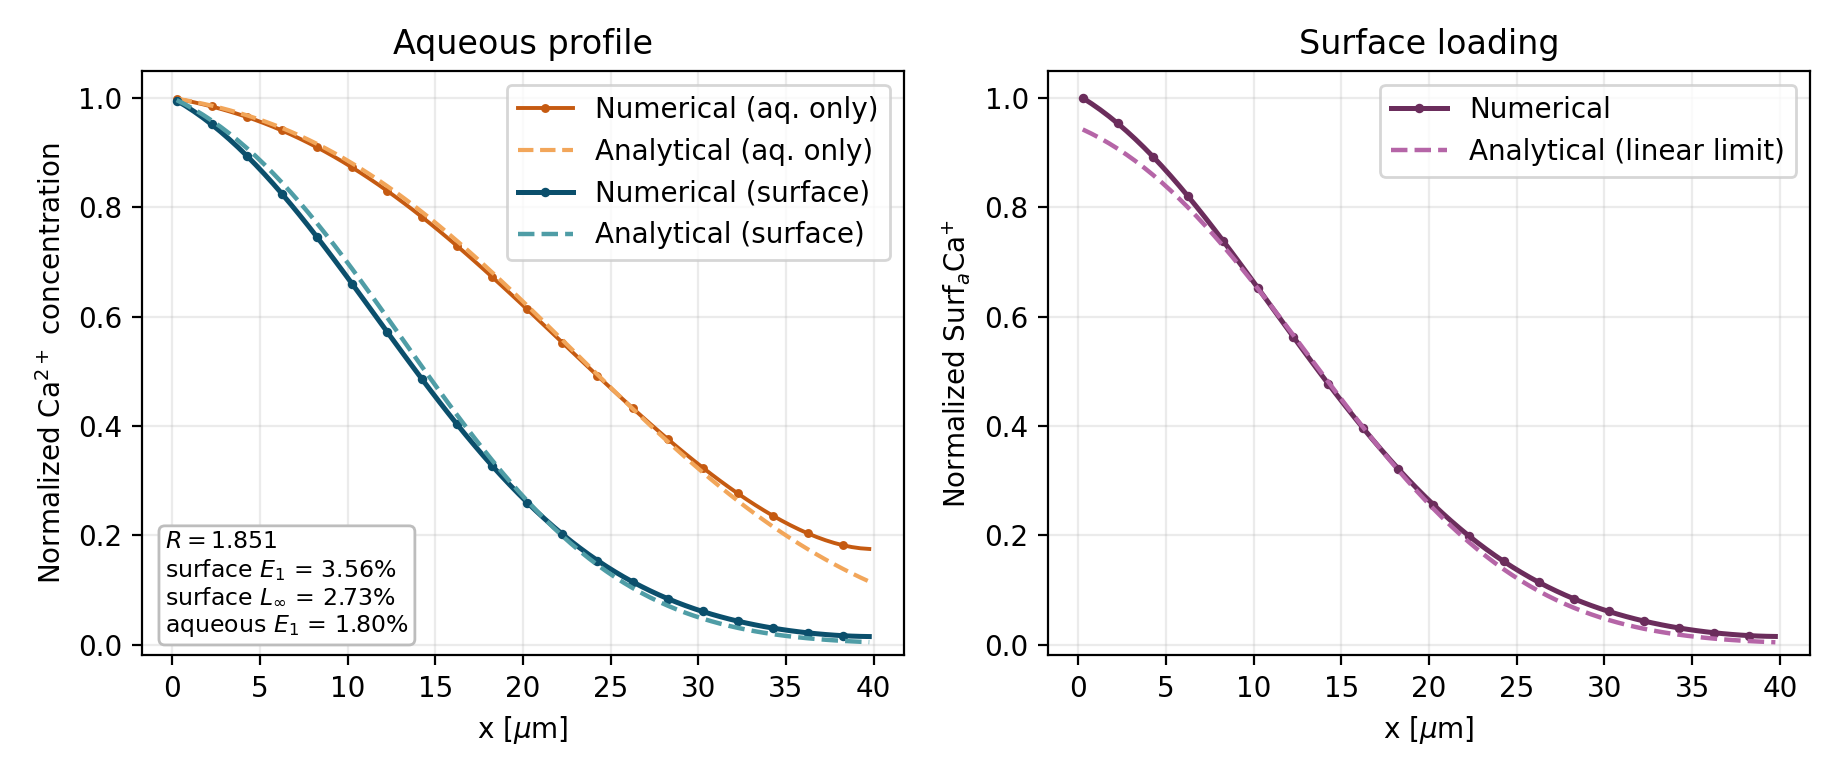
\includegraphics[width=0.9\linewidth]{figures/png/fig01_1d_retardation.png}
    \caption{1D analytical retardation benchmark. Left: normalized aqueous
    Ca$^{2+}$ profiles for the aqueous-only and surface-enabled runs, compared
    against their matching smooth advection-diffusion analytical solutions.
    Right: normalized surface loading compared against the linear-equilibrium
    analytical limit constructed from the calibrated field-level
    $K_{s,\mathrm{field}}$.}
\end{figure}

\subsection{Controlled Numerical Validation}

In addition to the analytical benchmark, the solver has been checked against a
set of controlled numerical baselines:
\begin{itemize}
\item aqueous-only reduction,
\item \mbox{$a_{\mathrm{surf}} = 0$} reduction,
\item closed-system adsorption and desorption,
\item decomposition, timestep, and mesh sensitivity on the fixed 1D benchmark.
\end{itemize}

These checks constrain both the mathematical correctness and the current
operating envelope used in the later image-based test cases.

\subsection{Validation Outputs Required For The Final Draft}

For the manuscript to be internally reviewable, the validation section should
end with a compact summary table containing:
\begin{itemize}
\item reduction-path pass/fail status,
\item analytical benchmark error,
\item decomposition sensitivity,
\item timestep sensitivity,
\item mesh sensitivity,
\item one representative chemistry-cost metric.
\end{itemize}

\begin{table}[htbp]
    \centering
    \caption{Placeholder for the validation summary table.}
    \begin{tabular}{lll}
        \toprule
        Check & Metric & Placeholder status \\
        \midrule
        Analytical 1D & Profile error / inventory drift & Drafted \\
        Decomposition & Total-equivalent drift & To be populated \\
        Timestep & Front-shape drift & To be populated \\
        Mesh & Front / total drift & To be populated \\
        Performance & Chemistry fraction & To be populated \\
        \bottomrule
    \end{tabular}
\end{table}

\section{Test Cases}

\begin{table}[htbp]
    \centering
    \caption{Planned test-case ladder for the manuscript.}
    \begin{tabular}{llll}
        \toprule
        Stage & Geometry source & Role & Planned output \\
        \midrule
        1D & tracked 1D benchmark & analytical limit & line/profile PNG \\
        2D & 4StraightFractures & transparent image case & 2D panel PNG \\
        3D & Kelvin1-200x200x200 & simple 3D topology & slice/render PNG \\
        3D large & Est\_3phase500cubed4micron & porous-media demo & multi-panel PNG \\
        \bottomrule
    \end{tabular}
\end{table}

\subsection{Simple 2D Image-Based Case}

The planned 2D case reuses the existing segmented image asset:
\begin{itemize}
\item \texttt{images/raw/4StraightFractures.raw.tar.gz}
\item metadata: \texttt{images/raw/4StraightFractures.txt}
\end{itemize}

This case should play the same role as the simple 2D case in the reference
paper: a geometrically transparent test that makes the coupling between
transport, internal surface interaction, and retardation easy to interpret.

Planned figure set:
\begin{itemize}
\item geometry PNG,
\item aqueous concentration PNG,
\item surface loading PNG.
\end{itemize}

The 2D case should be written to answer three questions:
\begin{enumerate}
\item does the method recover the expected directional retardation pattern in a
simple geometry,
\item does the surface-loading field track the geometry in an interpretable
way,
\item does the 2D image case remain visually and numerically easier to audit
than the 3D cases.
\end{enumerate}

\subsection{Simple 3D Image-Based Case}

The planned simple 3D case reuses:
\begin{itemize}
\item \texttt{images/raw/Kelvin1-200x200x200.raw.tar.gz}
\item metadata: \texttt{images/raw/Kelvin1-200x200x200.txt}
\end{itemize}

This case should demonstrate the transition from 2D transport pathways to a
fully 3D unresolved surface network while still remaining easy to interpret.

The simple 3D section should focus on:
\begin{itemize}
\item how 3D topology changes the transport path,
\item how the unresolved internal surface distribution changes the uptake
pattern,
\item how much the 3D case increases chemistry cost relative to the 2D case.
\end{itemize}

\subsection{Large 3D Porous-Media Case}

The planned large 3D porous-media case reuses:
\begin{itemize}
\item \texttt{images/raw/Est\_3phase500cubed4micron.raw.tar.gz}
\item metadata: \texttt{images/raw/Est\_3phase500cubed4micron.txt}
\end{itemize}

This case is the application-scale demonstration. It should use an
Estaillades-style multi-scale image so the method is exercised on a domain with
more realistic multi-scale structural contrast than the controlled 2D and
simple 3D cases.

The large porous-media section should report:
\begin{itemize}
\item mesh/image size,
\item effective resolution,
\item visible multi-scale structural contrast in the reported slices,
\item MPI rank count,
\item representative runtime,
\item one concentration metric and one surface-loading metric that remain
comparable to the earlier sections.
\end{itemize}

\begin{figure}[htbp]
    \centering
    \fbox{\rule{0pt}{2in}\rule{0.9\linewidth}{0pt}}
    \caption{Placeholder for the 2D case figure set
    (planned PNG target: \texttt{figures/png/fig02\_2d\_fractures.png}).}
\end{figure}

\begin{figure}[htbp]
    \centering
    \fbox{\rule{0pt}{2in}\rule{0.9\linewidth}{0pt}}
    \caption{Placeholder for the simple 3D case figure set
    (planned PNG target: \texttt{figures/png/fig03\_3d\_kelvin.png}).}
\end{figure}

\begin{figure}[htbp]
    \centering
    \fbox{\rule{0pt}{2in}\rule{0.9\linewidth}{0pt}}
    \caption{Placeholder for the large 3D porous-media Estaillades case figure
    set (planned PNG target: \texttt{figures/png/fig04\_3d\_estaillades.png}).}
\end{figure}

\section{Discussion}

\subsection{Formulation Choices and Conservative Structure}

The central modelling choice in this work is to use one fixed porosity field,
$\theta$, in the finite-volume transport equation and in the PHREEQC cell
volumes alike, which keeps aqueous accumulation, transport, and equilibrium
chemistry on the same volumetric basis. The reactive surface is prescribed
independently through the explicit cell field $a_{\mathrm{surf}}$, so the
chemical storage volume and the amount of reactive surface remain separately
defined material properties.

This approach extends earlier micro-continuum reactive transport formulations
to the case where the reactive surface area is an unresolved cell property
rather than an explicitly meshed boundary. In existing pore-scale DBS solvers,
including \nolinkurl{porousMedia4Foam} and earlier GeoChemFoam solvers,
reactive uptake is typically imposed as a flux condition on the diffuse
fluid-solid interface. This requires the reactive surface to coincide with the resolved image voxel
boundary, which is a good approximation when the dominant reactive area lies at
the contact between macropore and grain. In multi-scale carbonate images the
microporous phase holds a large internal reactive area that lies inside the
coarse cell rather than on its boundary. The cell-based formulation carries
that area as an intrinsic volumetric density
$a_{\mathrm{surf}}^{\mathrm{intrinsic}}$, scaled by the local phase fraction
and passed to PHREEQC as a cell-level property.

The closed-batch balance isolates the round-trip transfer of aqueous and
adsorbed Ca between the finite-volume fields and PhreeqcRM: with transport and
boundary fluxes disabled, the combined inventory
$M=\theta C+a_{\mathrm{surf}}\Gamma$ should remain unchanged during local
equilibration. The transient 1D benchmark then tests the coupled transport
response, while its mesh- and timestep-refinement study quantifies the combined
spatial, temporal, and sequential-coupling errors.

\subsection{Geometric Scalability}

Because the validation ladder separates aqueous--surface state transfer,
coupled transport, surface-area geometry, and microporosity, the evidence can
be attributed to the layer that produced it. The closed-batch residual remains
below $10^{-9}$ in relative magnitude, the reported transient profiles differ
from the finest combined result by $3.01\%$ and $1.05\%$ for the
surface-enabled and aqueous-only cases, and the interface-area construction is
accurate to sub-percent levels against analytic spheres at
$R/\Delta x\ge16$ and against circular posts at all four tested resolutions. The
intrinsic micropore density enters only in the cases that use it.

The transition from 2D to 3D introduces qualitatively different transport paths
and surface-loading distributions. In the 2D case, open fractures provide
preferential pathways for dissolved Pb$^{2+}$, while strong-site Pb occupancy
varies across the surrounding microporous matrix and is enhanced near the inlet
and fracture intersections. In the 3D cases, the tortuosity of the
pore network produces a more dispersed front and a more heterogeneous
surface-loading pattern. This spatial heterogeneity in surface uptake controls the effective retardation
factor seen at the continuum scale, and following it requires a simulation that
resolves the local connectivity of the image.

The direct resolved-to-DBS comparison spans $Pe=0.1$ to $10$, with no
observed breakdown in agreement at the higher $Pe$ values tested. This
behaviour is consistent with the spatially uniform matrix closure and
repeated geometry of the benchmark, whose limited heterogeneity may help
preserve the accuracy of the two-scale representation as advection becomes
more dominant.

\subsection{Computational Cost Drivers}

PHREEQC is called once per active cell per timestep, with a full speciation
and surface-equilibration calculation for each cell. The chemistry overhead
therefore depends primarily on the number of active cells, the geochemical
system, and the frequency of the chemistry call. The resolved-wall and DBS
comparisons use the same nominal image resolution and quantify physical
agreement. A controlled performance comparison across resolutions is outside
the scope of this study. For larger grids or more complex geochemical systems,
masking near-solid cells
out of the PhreeqcRM mapping (here at
$\theta \le \theta_{\mathrm{mask}} = 10^{-3}$) is the main lever on that cost.
The threshold is held fixed across all examples here.

\subsection{Limitations and Future Work}

The intrinsic micropore end member $s_{\mathrm{micro}}$ is prescribed from
complementary measurements such as nitrogen BET adsorption, mercury intrusion
porosimetry, or finer-resolution image analysis \citep{noiriel2009changes}.
The segmented image determines the geometric fraction $f_{\mathrm{micro}}$,
and their product gives the bulk-volume cell contribution
$a_{\mathrm{surf}}^{\mathrm{intrinsic}}=f_{\mathrm{micro}}s_{\mathrm{micro}}$.
Uncertainty in $s_{\mathrm{micro}}$ is therefore a leading physical uncertainty
in microporous applications. This uncertainty is not specific to the
cell-based formulation: a resolved-wall representation constructed from the
same segmented image also cannot recover reactive area below the image
resolution without complementary characterisation. Linking image-derived
phase fractions to measured or computed phase-specific surface densities is
therefore required to constrain predicted uptake.

The upscaled DBS treatment carries unresolved matrix properties as local
cell-averaged quantities. When diffusive exchange is fast compared with the
advective residence time, the intrinsic surface area acts as a locally
accessible reactive reservoir. At larger $Pe$, advective bypass and finite
matrix-exchange times can restrict access to that area, so reactive uptake
depends on its time-dependent accessibility as well as its amount. This
transport-upscaling limitation is distinct from the assumption of local
chemical equilibrium within each active cell: local equilibration does not
ensure that solute reaches the unresolved reactive surface. Media with more
heterogeneous matrix properties, connectivity, or exchange length scales
therefore require their own $Pe$-resolved assessment.

The resolved-to-DBS comparison tests this practical consequence of the
intrinsic-area representation directly. For this micromodel, the small
inventory differences and modest axial-profile differences show that replacing
explicitly resolved matrix pore walls with cell-supported reactive area does
not materially alter domain-scale Li uptake across the tested $Pe$ range.

Transport and chemistry are coupled by a first-order Lie splitting, which
introduces a splitting error that scales with the timestep and the stiffness of
the reaction terms. For the surface-complexation systems used here, that error
sits within the benchmark agreement reported in Section~\ref{sec:validation},
but it may become significant for faster reactions or stiffer geochemical
systems. A second-order Strang splitting \citep{strang1968construction} is the
natural extension.

Restart depends on the serialised PHREEQC state written with each complete
checkpoint, because the finite-volume \texttt{Surf\_*} fields alone cannot
reconstruct that state. The production $Pe$ sweep restarted from these
checkpoints across several jobs, and moving a run between machines requires the
field data and its matching PHREEQC dump to travel together.

The cases here use a fixed surface area and equilibrium surface complexation,
and cover competitive multi-component chemistry and a Li-selective multi-ion
brine within that scope. Evolving reactive area, mineral dissolution and
precipitation, kinetic surface reactions, and the wider range of mineral
surfaces and aqueous compositions found in natural systems lie outside it.
Extending the model to them will require benchmarks that separate transport
error, surface-area evolution, and reaction-model uncertainty while retaining
cell-level mass-balance checks.

\section{Conclusions}

This work presents a conservative DBS formulation for PHREEQC-coupled reactive
transport with cell-based surface complexation in image-based porous media,
validated across analytical, image-based, and multi-scale porous-media cases.

The key contribution is a cell-based representation of unresolved reactive
surface area that sits inside the DBS micro-continuum framework. One fixed
porosity field serves aqueous accumulation, transport, and the PHREEQC cell
volumes alike, which keeps the aqueous transport conservative and the local
mass balance closed cell by cell. The unresolved micropore surface enters as an
additive intrinsic volumetric density, so reactive uptake can be represented in
image phases whose internal surface area lies inside the coarse cell rather
than on its boundary.

The 1D tests preserve the closed-batch Ca inventory to a relative residual
below $10^{-9}$ and show approximately first-order mesh and timestep
convergence, while the surface-area reconstruction recovers analytic interface
area to sub-percent accuracy for 3D spheres at $R/\Delta x\ge16$ and
quasi-2D circular posts at all four tested resolutions. In the Li micromodel, the
intrinsic-area representation keeps both aqueous and sorbed inventories within
$0.6\%$ of the resolved result over $Pe=0.1$--10, while the sorbed streamwise
profile differs by up to $4.75\%$. Across the 2D and 3D image-based cases, the
model resolves the dissolved and adsorbed fields that follow from the local
pore geometry and competition between species for surface sites.

Surface complexation can therefore be carried conservatively on cells whose
reactive area is unresolved, freeing the reactive surface from the resolved
mesh boundary in multi-scale image-based simulation. This matters for reactive
porous-media problems in which selectivity and surface accessibility control
performance, among them contaminant retention, radionuclide migration, and
critical-mineral recovery by sorbent-bearing porous media. Constraining the intrinsic surface-area input against measured internal area is
the step that would most improve predictive accuracy, and extending the
formulation to evolving reactive area and kinetic surface chemistry would open
the dissolution and precipitation problems that the equilibrium treatment
excludes.


\section*{Supplementary Information}

\textbf{Online Resource 1: Supplementary methods and validation.}
The resource contains the one-dimensional mesh and timestep convergence
study, reactive-area construction and capacity mapping, discrete PhreeqcRM
coupling and checkpoint restoration, short two-scale reconstruction
sensitivity, and reproducibility and data-provenance information.

\backmatter

\bibliography{references}

\section*{Statements and Declarations}

\textbf{Funding:} This work was supported by the Natural Environment Research
Council (NERC) and Nuclear Waste Services (NWS) through the GeoSAFE grant
(reference NE/Y002504/1). Opinions, findings, conclusions or recommendations
expressed are those of the authors and do not necessarily reflect the views
of NERC or NWS.

\textbf{Competing interests:} The authors have no relevant financial or
non-financial interests to disclose.

\textbf{Ethics approval:} Not applicable.

\textbf{Consent to participate:} Not applicable.

\textbf{Consent for publication:} Not applicable.

\textbf{Availability of data and materials:} The data and materials supporting
this study are available from the corresponding author on reasonable request.

\textbf{Code availability:} The GeoChemFoam 5.2 codebase is publicly available
at \url{https://github.com/GeoChemFoam/GeoChemFoam-5.2}. The solver modifications,
paper-specific cases, simulation scripts, and post-processing code are available
from the corresponding author on reasonable request.

\textbf{Authors' contributions:} \textbf{Hannah P. Menke:} Conceptualisation,
Methodology, Software, Investigation, Formal analysis, Writing -- original
draft, Funding acquisition. \textbf{Julien Maes:} Conceptualisation,
Methodology, Writing -- review \& editing, Funding acquisition.
\textbf{Florian Doster:} Conceptualisation, Writing -- review \& editing,
Funding acquisition.

\end{document}
